\documentclass{article}
\usepackage{graphicx}
\usepackage{caption}
\usepackage{svg}
\usepackage{subcaption}
\usepackage{hyperref}
\usepackage{cleveref}
\usepackage{adjustbox}
\usepackage{listings}

\lstset{
	breaklines=true
}

\graphicspath{{./images/}}

\hypersetup{
    colorlinks=true,
    linkcolor=blue,
    filecolor=magenta,      
    urlcolor=cyan,
    pdftitle={Presentation},
    pdfpagemode=FullScreen,
}

\title{h550 project - Security assessment of an AP}
\author{Esteban Aguililla Klein}
\begin{document}
\maketitle	
\tableofcontents
\newpage
\section{Abstract}
Closed source firmware cannot be trusted. Therefore, we will show how to hack an access point and search for exploitable vulnerabilities from the hardware to the software. Doing, so we will take a look at how U-boot and BusyBox shells can be used and leveraged to our advantage. Afterwards, we will showcase a level 10\footnote{\url{https://nvd.nist.gov/vuln/detail/CVE-2014-0659}} known vulnerability (which is in fact a backdoor placed by the constructor) that allows remote code execution and how it was found. 
\section{Introduction}
Nowadays most IOT devices contain some flavor of a vulnerability, backdoor or critical bug. However, those problems in some cases are never fixed as IoT devices are dependent on their vendors for firmware update due their code being proprietary (in most cases). Furthermore, some users might forget (or not know) that their device's software is not updated and by extension, vulnerable. This paper takes the approach of a guide on how to perform basic hardware hacking on everyday embedded devices. What should be taken away from this work is the process which aims to be as generic as possible and not the results as the chosen target is now discontinued and irrelevant. Therefore, we will start by setting the scope of our analysis then, do reconnaissance under those constraints followed by the exploitation of our findings.
\section{Scope}
The device is an access point from Cisco released in October 2008, aimed at small businesses. This products has been discontinued in 2019 and its sales ended back in 2014.
\begin{figure}[!h]
	\centering
	\begin{subfigure}{0.3\textwidth}
		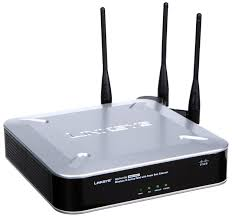
\includegraphics[width=\textwidth]{AP.jpg}
		\caption{Product picture}
		\label{outside}
	\end{subfigure}
	\begin{subfigure}{0.3\textwidth}
		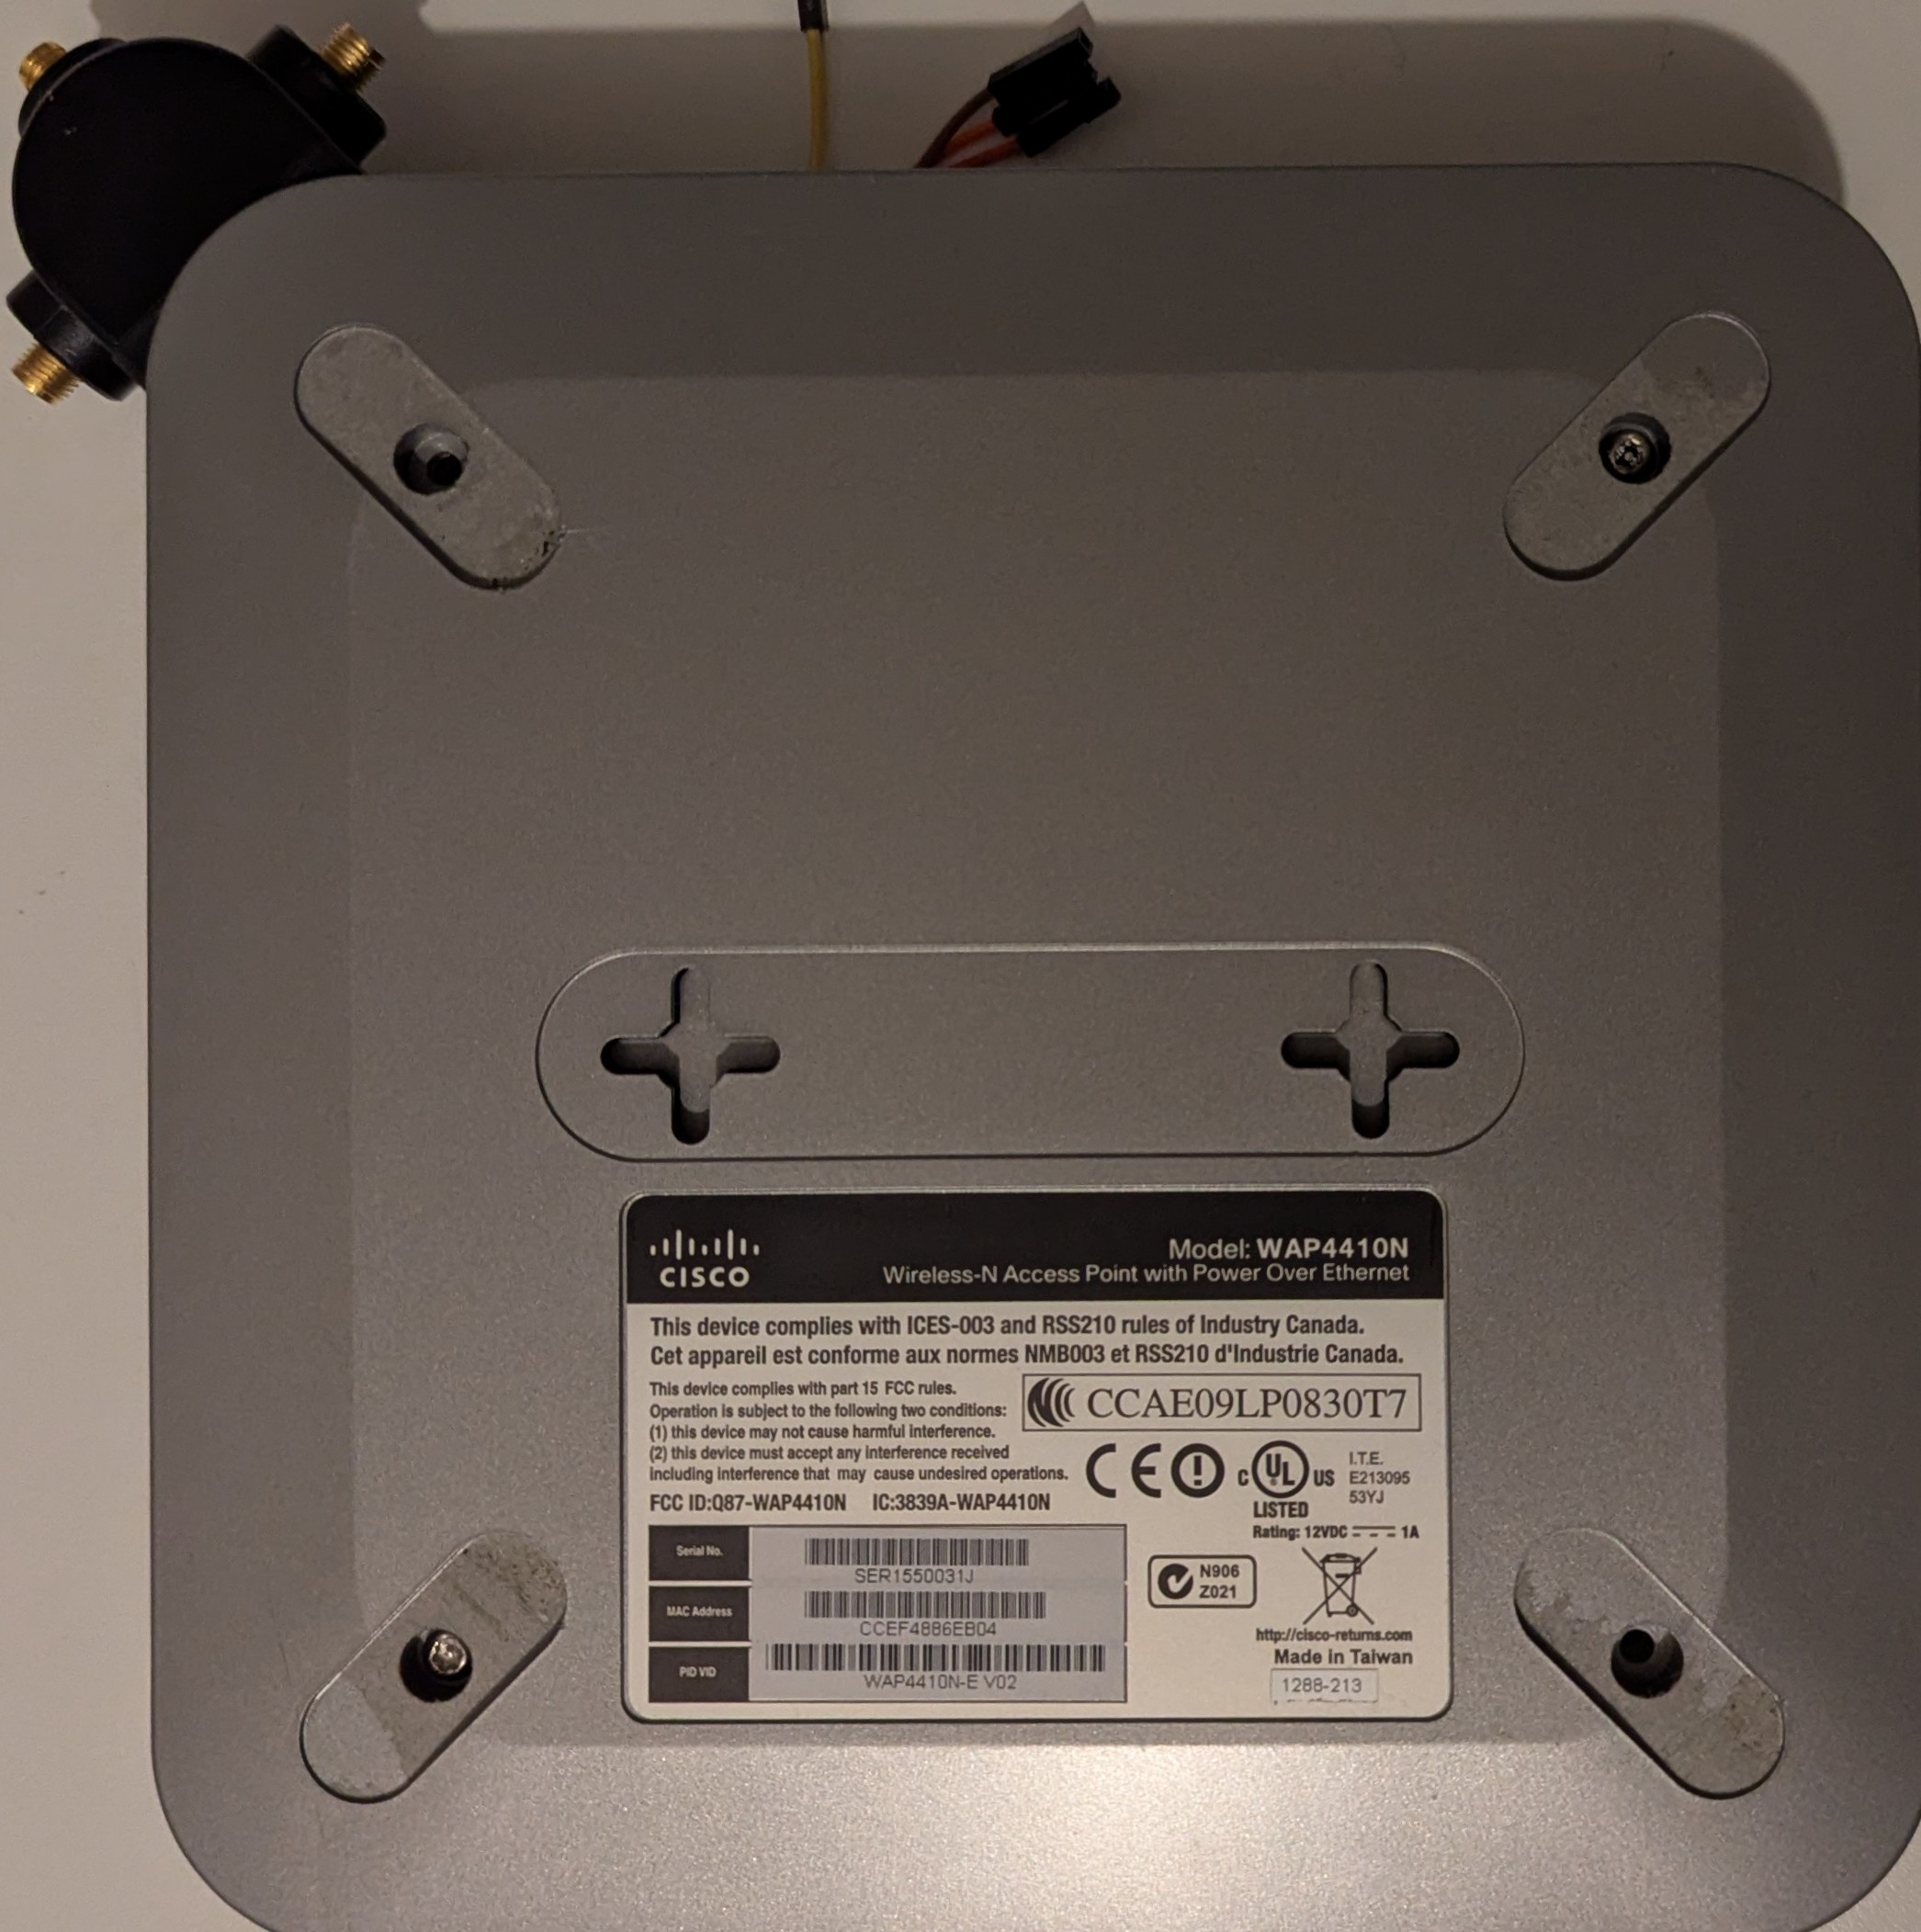
\includegraphics[width=\textwidth]{bottom.jpg}
		\caption{Bottom}
		\label{bottom}
	\end{subfigure}
	\begin{subfigure}{0.3\textwidth}
		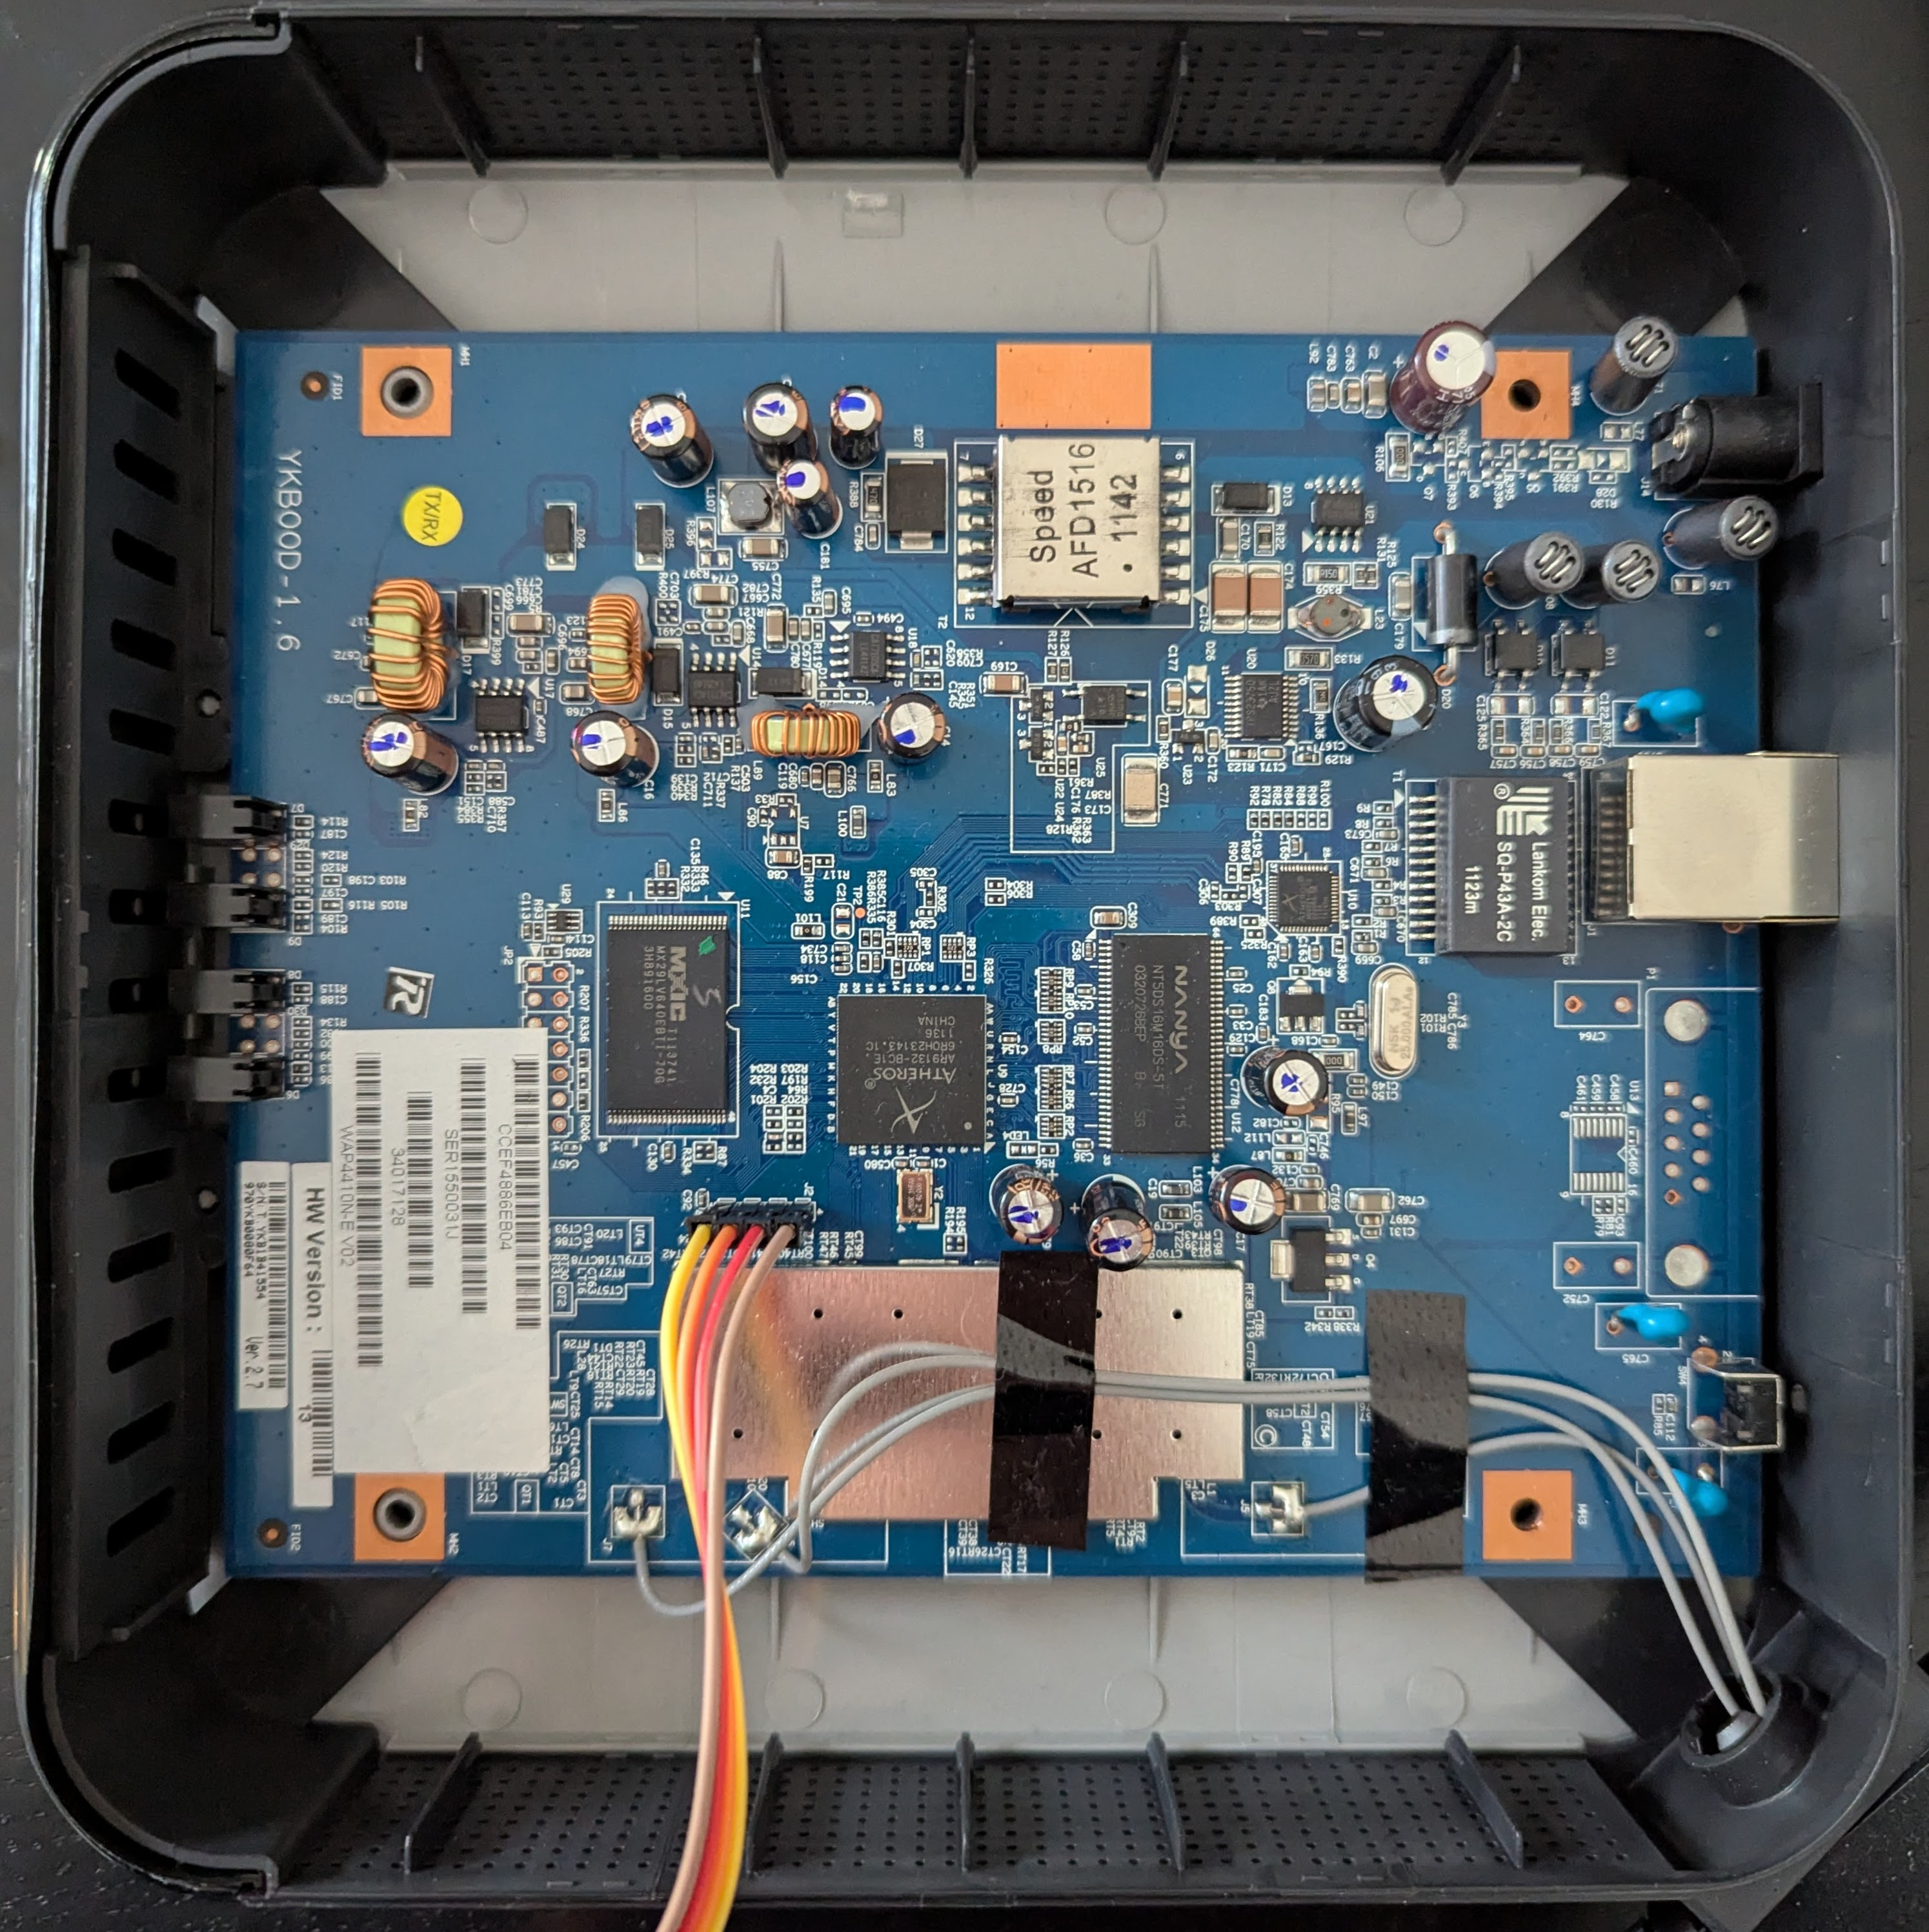
\includegraphics[width=\textwidth]{inside.jpg}
		\caption{Inside}
		\label{inside}
	\end{subfigure}
	\caption{Pictures of of the WAP4410N}
	\label{wap4410n}
\end{figure}

The device can be powered up using a barrel adapter or through PoE which hints at its purpose being ease of batch deployment. On the network side, it support 802.11n, 802.11g and 802.11b. With the time period in mind, for 802.11b and g, the only supported encryption protocol was WEP (64/128 bits in this case). Also, firmware updates were handled through the web porta : there is no I/O on the device. On figure \ref{inside}, we can see a cable going outside of the device, this is the UART access which was enabled by default.
\subsection{Lab setup}
The testing setup is made of the WAP4410N, a router and a computer : for simplicity sake, the router is out of scope from this analysis and all its security features are disabled. The computer has a wireless connection to the AP.
\begin{figure}[!ht]
	\includesvg[width=\textwidth]{images/lab.svg}	
	\caption{Lab setup}
\end{figure}
\subsubsection{Equipment}
The following table contains all the software and hardware required for basic hardware hacking. 
\begin{figure}[!ht]
\begin{tabular}{|c|c|}
	\hline
	software & hardware \\
	\hline
	Wireshark, nmap & FT232 board USB-A UART adapter \\
	GNU Screen, xxd, dd, binwalk &  Multimeter \\
	squashfs-utils & Dupont Cables \\
	radare2, ghidra & \\
	\hline
\end{tabular}
\caption{List of used software/hardware}
\end{figure}


At first, we intended to use a SPI programmer (CH341a) to dump the firmware more easily using \href{https://github.com/flashrom/flashrom}{flashrom}. However, as we will see in a later section, it was not feasible in this context without specialized hardware tools. On the software side, there are no real limitations as most of the state of the art tools are free and open source (with the exception of IDA).
\section{Reconnaissance}
This section was inspired by one of the steps cyber kill chain which will vaguely be followed throughout this paper. This is the most important part of any hardware hacking project : the more information about the target we have the easier finding vulnerabilities will become.
\subsection{Physical}
\paragraph{Teardown} The device is held together by four 8-points screws under rubber feets which indicates that it wasn't meant to be opened (nor repaired \dots). Once inside, most of the device is empty and everything is available without further need to dismantle it. 

\paragraph{IC reconnaissance} At this point we can start looking for interesting ICs like flash memory or processors :

\\
\begin{minipage}[t]{0.3\textwidth}
	\adjustimage{angle=90, valign=t}{images/flash.png}
\end{minipage} %
\vspace{0.5cm}
\hfill
\begin{minipage}[t]{0.7\textwidth}
	\begin{itemize}
		\itemsep0em
		\item reference : \href{https://www.alldatasheet.com/datasheet-pdf/view/267962/MCNIX/MX29LV640DBTC-90G.html}{MX29LV640DBTC-90G}
		\item format : 48 TSOP
		\item manufacturer : Macronix
		\item size : ~8MB
	\end{itemize}
\end{minipage}
\begin{minipage}[t]{0.3\textwidth}
	\adjustimage{width=\textwidth, angle=180, valign=t}{images/cpu.png}
\end{minipage} %
\vspace{0.5cm}
\hfill
\begin{minipage}[t]{0.7\textwidth}
	\begin{itemize}
		\item family : Atheros 9100
		\item reference : Atheros9132
		\item manufacturer : Qualcomm
		\item architecture : MIPS 24K V7.4 32bits
		\item endianness : big endian
		\item bogomips : 265.21
	\end{itemize}
\end{minipage}
\noindent The MIPS architecture is very common on embedded devices and very easy to reverse engineer its assembly. However, this makes it impossible for us to use frida as MIPS is only available in the pro version. Then, regarding the NAND flash, as hinted before, reading a 48 TSOP IC requires specialised and expensive hardware. Therefore, using an SPI programmer to dump it is out of the question.
\paragraph{Finding the UART} This is the most important step of the physical reconnaissance : the UART allows us to communicate with the device from a computer. To find it, we have to usually look for 3 to 4 pins next to each other. 

\begin{figure}[!ht]
	\includesvg[width=\textwidth]{images/uart.svg}
	\caption{UART connected through Dupont cables with labeled ports}
\end{figure}
\newpage

\noindent On the device, there are 4 male header pins that might be the UART. We can check using a multimeter. First, we must find the ground, to do so, we can look at any IC datasheet and find a ground pin then, we can try to find a grounded metal to connect to it instead of a pin by checking for continuity. After having found a ground connection we can start taking measurements of our candidate,
\begin{figure}[!ht]
	\centering
	\begin{tabular}{|c|c|c|c|}
		\hline
		pin & $R_{VSS}$ & $V$ & info \\ 
		\hline
		1 & $8.6k\Omega$ & $\approx 3.3V$ & VCC \\
		2 & $\infty k\Omega$ & $\approx 0V - VCC$ & TX\\
		3 & $\infty k\Omega$ & $\approx 0V$ & RX \\
		4 & $0$ k $\Omega$ & $0V$ & GND \\
		\hline
	\end{tabular}
	\caption{Multimeter measurements}
\end{figure}

\noindent The voltage goes from 0V to VCC, at startup because of the boot log outputs a lot of data. The RX has a voltage of 0 as its used to receive data and doesn't send any. The next step is to try connecting the UART to the computer using our TTL, 
\begin{figure}[!ht]
	\centering
	\includesvg[width=\textwidth]{images/ft232.svg}
	\caption{UART to USB-A }
\end{figure}

\noident Regarding the baudrate, we can try 115200 as its the most common value,
\begin{lstlisting}
	screen /dev/ttyUSB0 115200
\end{lstlisting} 
This is indeed the correct baudrate however, if that wasn't the case we would have had to find it by trial and error or by using a logic analyzer.
\subsection{Bootloader}
\subsubsection{Boot log}
First, we will take a look at the boot log that is displayed before getting access to any console as analyzing it provides a lot of information about the hardware, software, ... One such information is the bootloader : U-Boot 1.1.4 which is a very common and open source bootloader. 
\begin{lstlisting}
arg 1: console=ttyS0,115200
arg 2: root=31:02
arg 3: rootfstype=jffs2
arg 4: init=/sbin/init
arg 5: mtdparts=ar9100-nor0:256k(u-boot),
	64k(u-boot-env),
	6464k(rootfs),
	1280k(uImage),
	64k(nvram),
	64k(calibration)
arg 6: mem=32M
\end{lstlisting}
From the capture snippet above we see that the rootfs uses jffs2 however, this is not the case.
\begin{lstlisting}
Kernel command line: console=ttyS0,
	115200 root=31:02 rootfstype=squashfs init=/sbin/init mtdparts=ar9100-nor0:256k(u-boot),
	64k(u-boot-env),
	6464k(rootfs),
	1280k(uImage),
	64k(nvram),
	64k(calibration) 
	mem=32M 	
\end{lstlisting}
This snippet comes after the previous ones and tells us that rootfs uses squashfs. This information can be confirmed later using the console and/or by analyzing the dumped firmware. Usually an embedded device has two file systems with overlayfs : the union of two filesystems where the lower is read only (squashfs) and the upper read write (jffs2) for persistency. However, the device only uses squashfs, the configuration files are saved on non volatile memory through a program found in $/usr/sbin/nvram$
\subsubsection{U-boot}\label{ubootinfo}
At some point we are prompted to interrupt the auto boot : by doing so, we get the U-boot console which allows us to get more information on the device,
\begin{lstlisting}
ar7100> bdinfo
...
flashstart  = 0xBF000000
flashsize   = 0x00800000
flashoffset = 0x0002F690
...
baudrate    = 115200 bps	
\end{lstlisting}
We now know the memory addresses of the start and of the flash storage : this will come handy during the firmware extraction in \ref{Dumpuboot}. There are other useful commands available to us such as tftpboot which allows us to boot over the network by serving an image on our computer. Assuming that the console is protected, this could allow us to get an unrestricted console by providing our own patched image (or using an open source one). Other than that, there are custom commands for testing purposes.
\subsection{Console}
If we leave the autoboot alone, we get into a root Linux ash shell. There are device specific CLI commands and a reduced busybox. There is a fwversion command which tell us that the firmware version is 2.0.4.2. As we are already root, we can't really do any privilege escalation. Furthermore, as the device only has a squashfs3 file system we can't get any persistency.
\subsection{Network}
We can run a port scan on the device using nmap, 

\begin{lstlisting}
Nmap scan report for wap86eb04 (192.168.1.3)  
Host is up (0.012s latency).  
Not shown: 65532 closed tcp ports (reset)  
PORT      STATE SERVICE  
80/tcp    open  http  
443/tcp   open  https  
32764/tcp open  unknown  
MAC Address: CC:EF:48:86:EB:04 (Cisco Systems)
\end{lstlisting}

The http(s) ports are used for the web administrative portals : when using the http web portal the credential are sent through base64. However, this isn't really a problem as the http port will most likely be disabled by any competent IT staff in real use cases
\section{Exploitation}
In this section we will see how to exploit the device
\subsection{Dumping the firmware}
\subsubsection{Through the bootloader}\label{Dumpuboot}
This is the most "classical" technique used to dump firmware because of its simplicity and lack of technical and material requirements. To perform it, we will leverage the memory display command using the addresse from \ref{ubootinfo} and capturing the output. The size is written in decimal and divided by 4 as it reads by blocks of dwords. When the read is done, the output has to be cleaned into a binary format (there is a script in the repo). However, this technique didn't work in our case. The reason, is unclear as the output is not entirely unreadable when using binwalk : some possible reasons might be,
\begin{itemize}
	\item glitchy cable
	\item this version of U-Boot has a problem with memory display
	\item out of bound area on the NAND flash
	\item endianness problem	
\end{itemize}
\subsubsection{Through the console}
To do so, we have to update the version of busybox : we will download precompiled busybox binary and serve it to our device through an ftp server. We download it in the /tmp directory as it the only location in a read only filesystem where we can write a file. From there, we use netcat to upload the mtd partitions : concatenate the partitions together to make the whole firmware image :

\begin{lstlisting}[
    basicstyle=\fontsize{5}{7}\selectfont\ttfamily
]
                  /home/aaaaaa/aaaaaaaaa/aaa/aaaaaaaaaaaa/dump/firmware2.0.4.2.bin
-----------------------------------------------------------------------------------------------------
DECIMAL                            HEXADECIMAL                        DESCRIPTION
-----------------------------------------------------------------------------------------------------
158992                             0x26D10                            CRC32 polynomial table, big 
                                                                      endian
327680                             0x50000                            SquashFS file system, big 
                                                                      endian, version: 3.0, 
                                                                      compression: unknown, inode 
                                                                      count: 794, block size: 65536, 
                                                                      image size: 4761817 bytes, 
                                                                      created: 2011-05-13 10:54:02
6946816                            0x6A0000                           uImage firmware image, header 
                                                                      size: 64 bytes, data size: 
                                                                      875547 bytes, compression: 
                                                                      gzip, CPU: MIPS32, OS: Linux, 
                                                                      image type: OS Kernel Image, 
                                                                      load address: 0x80002000, 
                                                                      entry point: 0x801C2000, 
                                                                      creation time: 2011-05-13 
                                                                      10:51:49, image name: "Linux 
                                                                      Kernel Image"
8269351                            0x7E2E27                           PEM private key
8270238                            0x7E319E                           PEM certificate
-----------------------------------------------------------------------------------------------------
\end{lstlisting}

with this we can do some reverse engineering however, as the rootfs uses squashfs3 we can't patch binaries on the fly : we need to upload the entire firmware therefore we didn't path any binary.
\subsection{CVE-2014-0659}
This \href{https://nvd.nist.gov/vuln/detail/CVE-2014-0659}{CVE} is a backdoor planted by SerComm. To try it, we ping the 32764 using netcat : this opens a prompt in which after entering some random data and press enter will answer with ScMM,
\begin{figure}[!ht]
	\centering
	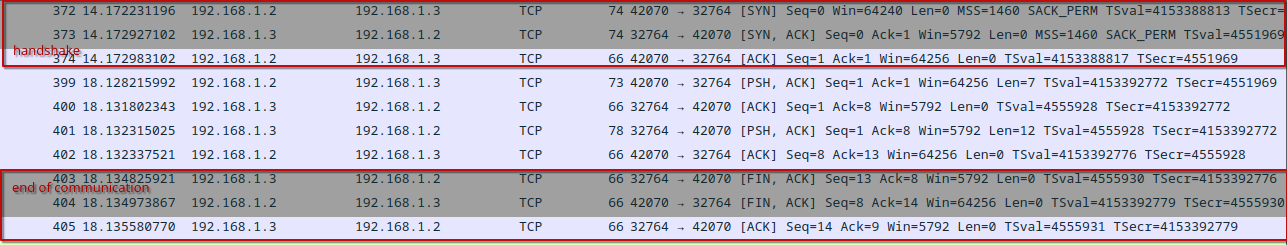
\includegraphics[width=\textwidth]{example.png}
	\caption{Capture of the exploit traffic}
\end{figure}
when analyzing the traffic we can notice the data that we sent and as the answer we get, 53 63 4d 4d ff ff ff ff 00 00 00 00 which translates to ScMM. Based on the work of \href{https://github.com/elvanderb/TCP-32764}{Eloi Vanderbken} : you can use this exploit to get remote code execution on the device. Going into some reverse engineering of the vulnerable binary.
\subsection{Reverse Engineering}
The vulnerability is located int he \textbf{scfgmgr} file : we know this because it mas mentioned by the discoverer of the vulnerability. However, to find it naturally, one can look at the process list and analyze all the programs that sound like they don't belong there. The backdoor opens a new child process for each new connection to its socket and starts an alarm of 10s during which you have to send the correct character sequence : 
\begin{enumerate}
	\item Checks if the response starts with the correct code \textit{(ScMM)} and is followed by and identifier ( we will call it \textbf{id} ) and optionally an argument
	\item The program matches the \textbf{id} and, if it matches with a known \textbf{id} it performs the corresponding action \textit{eg. there is an id for restarting the device}
	\item The child process terminates
\end{enumerate}

One of those \textit{id}, opens a pipe that calls for \textbf{popen} with the user input as argument and returns the output through the socket.
\begin{figure}[!ht]
	\begin{lstlisting}[language=c]
	  read_ret = (char *)malloc(1);
	  *read_ret = '\0';
	  *output = read_ret;
	  __stream = popen(command,"r");	
	\end{lstlisting}
	\caption{Snippet of vulnerable code}	
\end{figure}
In the snippet above, \textbf{command} is a user input and, the resulting stream from the \textbf{popen} command is read into the \textbf{read\_ret} which is pointed by \textbf{output} : a function argument. After, returning from the pipe, \textbf{output} is written to the socket.


\end{document}

